\documentclass{article}

\usepackage[margin=1.0in]{geometry}
\usepackage{graphicx}

\title{Improving Object Characteristic Enumeration Models with Transfer Learning and Data Augmentation}
\date{4/20/2018}
\author{Simon Swenson}

\begin{document}

\maketitle
\pagenumbering{gobble}
\newpage
\pagenumbering{arabic}

\section{Abstract}

Transfer learning is an important, growing area of deep learning research. Many ready-to-use networks exist on the internet and with pre-trained weights. One of our goals was to leverage that ever-growing set of ready-to-use networks, specifically image classification networks, and use them for generating sets of characteristics for an object from an image of that object.

We gathered a set of simple objects with known characteristics (like "blue" or "cube") and with some overlap in the characteristics (like a blue cube, a blue cylinder, and a red cube). To improve our model's understanding of the objects, we captured images of those objects in a variety of environments from a variety of angles.

To test if the models truly understood the objects and the corresponding characteristics, we introduced several test sets, (1) the training objects in a different environment, (2) objects which shared some characteristics of the training objects in the same environment(s), and (3) objects which shared some characteristics of the training objects in a different environment.

Our findings were that many model configurations descended to the all 0's output model. We observed that, as the number of neurons per layer and number of densely connected layers in our network increased, the probability of descending to the all-0's output model approached 1. However, some model configurations were able to improve accuracy on the training data, but no model was able to find any connection between the training data and testing data; as the training accuracy increased, test accuracy was immediately inversely affected. Possible reasons are given in the "Conclusion" section.

\section{Introduction}

Though most interest in image processing applications has been directed toward one of:

\begin{itemize}
	\item Object detection
	\item Object classification
	\item Image captioning
\end{itemize}

an important task for understanding objects as they are is to understand the characteristics of that object and be able to abstract those characteristics and apply them to other, somewhat related, objects. For example, after seeing enough instances of objects which have a characteristic of "blue," one might come to an understanding of that characteristic and would thus be able to apply the characteristic "blue" to other blue objects that one has never experienced prior. This ability is essential for robots and AI agents, as it allows them to apply their understanding of previous objects to new objects.

Such a task can be quite difficult, and a large, complicated neural network may be required for it. However, many ready-to-use models with pre-computed weights exist in libraries such as Keras. As the task outlined above requires image processing, the relevant ready-to-use models must also take image data as an input. Image classification networks, such as "Xception," are promising in that regard, and we opted to make use of them.

In addition to such transfer learning, we can turn to the human learning process to inform us on how to proceed. One method that humans often use to learn about new objects is to examine them from a variety of different angles. Thus, such an approach seemed promising for this task.

\section{Architecture}

Let:

\begin{itemize}
	\item $ O = \{o_1, o_2, ..., o_n\} $ be the set of objects to be considered
	\item $ O_{tr} \subseteq O $ be the set of train objects
	\item $ O_{te} \subseteq O $ be the set of test objects with $ O_{tr} \cap O_{te} = \emptyset $
	\item $ c $ be a set, the corpus of characteristics found among training objects for this session
	\item $ C: O \rightarrow \wp(c) $ be a mapping from objects to their associated characteristics.
	\item $ L = \{l_1, l_2, ..., l_m\} $ be the set of locations in the world at which to capture objects
	\item $ L_{tr} \subseteq L $ be the set of train locations
	\item $ L_{te} \subseteq L $ be the set of test locations with $ L_{tr} \cap L_{te} = \emptyset $
	\item $ P $ be a set of two-tuples, a rotation and a translation from which the objects will be captured at each location
\end{itemize}

Then we can define the image capture, $ I $, as a mapping $ I: O \times L \times P \rightarrow R^{q \times r} $, for some $ q, r $. Our goal is then to find the mapping $ M: R^{q \times r} \rightarrow \wp(c) $ such that $ \forall o \in O, l \in L, p \in P, M(I(o, l, p)) = C(o) $. However, using transfer learning requires us to not only find one mapping $ M $, but two models $ Mo_1, Mo_2 | M = Mo_2 \circ Mo_1  $.

\subsection{Test Criteria}

An important part of this task is defining what, exactly, to test, as it will determine the exact architecture for the solution. For this task, we decided to measure the success of the model in three different ways:

\begin{enumerate}
	\item Given an image of an object:
	\begin{enumerate}
		\item in the set of training objects but 
		\item in a different environment from the training environments
	\end{enumerate}
	can the network produce the correct characteristics for that object?
	\item Given an image of an object:
	\begin{enumerate}
		\item not in the set of training objects but
		\item in an environment in the set of training environments and
		\item sharing at least one characteristic with an object in the set of training objects
	\end{enumerate}
	can the network produce the correct characteristics for that object?
	\item Given an image of an object
	\begin{enumerate}
		\item not in the set of training objects and
		\item in an environment in the set of training environments and
		\item sharing at least one characteristic with an object in the set of training objects
	\end{enumerate}
	can the network produce the correct characteristics for that object?
\end{enumerate}

In formal terms, we measure success by computing the accuracy of our model, $ Mo_2 $ using the following three metrics:

\begin{enumerate}
	\item $ Accur_{Te_{1}} = \frac {\sum_{o \in O_{tr}} \sum_{l \in L_{te}} \sum_{p \in P} |c| - | Mo_2(Mo_1(I(o, l, p))) \oplus C(o) |} {|O_{tr}| \dot |L_{te}| \dot |P| \dot |c| } $
	\item $ Accur_{Te_{2}} = \frac {\sum_{o \in O_{te}} \sum_{l \in L_{tr}} \sum_{p \in P} |c| - | Mo_2(Mo_1(I(o, l, p))) \oplus C(o) |} {|O_{te}| \dot |L_{tr}| \dot |P| \dot |c| } $
	\item $ Accur_{Te_{3}} = \frac {\sum_{o \in O_{te}} \sum_{l \in L_{te}} \sum_{p \in P} |c| - | Mo_2(Mo_1(I(o, l, p))) \oplus C(o) |} {|O_{te}| \dot |L_{te}| \dot |P| \dot |c| } $
\end{enumerate}

\section{Implementation}

\subsection{Data Acquisition}

We used the following objects for training and testing.:

\begin{tabular}{r | c c c | l | l }
	Obj & Shape & Dimensions & Color & Characteristics & Te/Tr \\
	\hline
	$ o_{bo} $ & Cone & d = 82.5 mm & Krylon Gloss & \{"blue", "cone"\} & Tr \\
	& & h = 82.5 mm & True Blue & & \\
	$ o_{bu} $ & Cube & w = 60 mm & Krylon Gloss & \{"blue", "cube"\} & Tr \\
	& & & True Blue & & \\
	$ o_{by} $ & Cylinder & d = 75 mm & Krylon Gloss & \{"blue", "cylinder"\} & Tr \\
	& & h = 50 mm & True Blue & & \\
	$ o_{ro} $ & Cone & d = 82.5 mm & Krylon Gloss & \{"red", "cone"\} & Tr \\
	& & h = 82.5 mm & Banner Red & & \\
	$ o_{ru} $ & Cube & w = 60 mm & Krylon Gloss & \{"red", "cube"\} & Tr \\
	& & & Banner Red & & \\
	$ o_{ry} $ & Cylinder & d = 75 mm & Krylon Gloss & \{"red", "cylinder"\} & Tr \\
	& & h = 50 mm & Banner Red & & \\
	$ o_{yo} $ & Cone & d = 82.5 mm & Krylon Gloss & \{"yellow", "cone"\} & Tr \\
	& & h = 82.5 mm & Sun Yellow & & \\
	$ o_{yu} $ & Cube & w = 60 mm & Krylon Gloss & \{"yellow", "cube"\} & Tr \\
	& & & Sun Yellow & & \\
	$ o_{yy} $ & Cylinder & d = 75 mm & Krylon Gloss & \{"yellow", "cylinder"\} & Tr \\
	& & h = 50 mm & Sun Yellow & & \\
	$ o_{yi} $ & Icosahedron & $ r_{flats} $ = 70 mm & Krylon Gloss & \{"yellow"\} & Te \\
	& & & Sun Yellow & & \\
	$ o_{wu} $ & Cube & w = 80 mm & Rust-oleum & \{"cube"\} & Te \\
	& & & Flat White & & \\
\end{tabular}

\begin{figure}[h!]
	\centering
	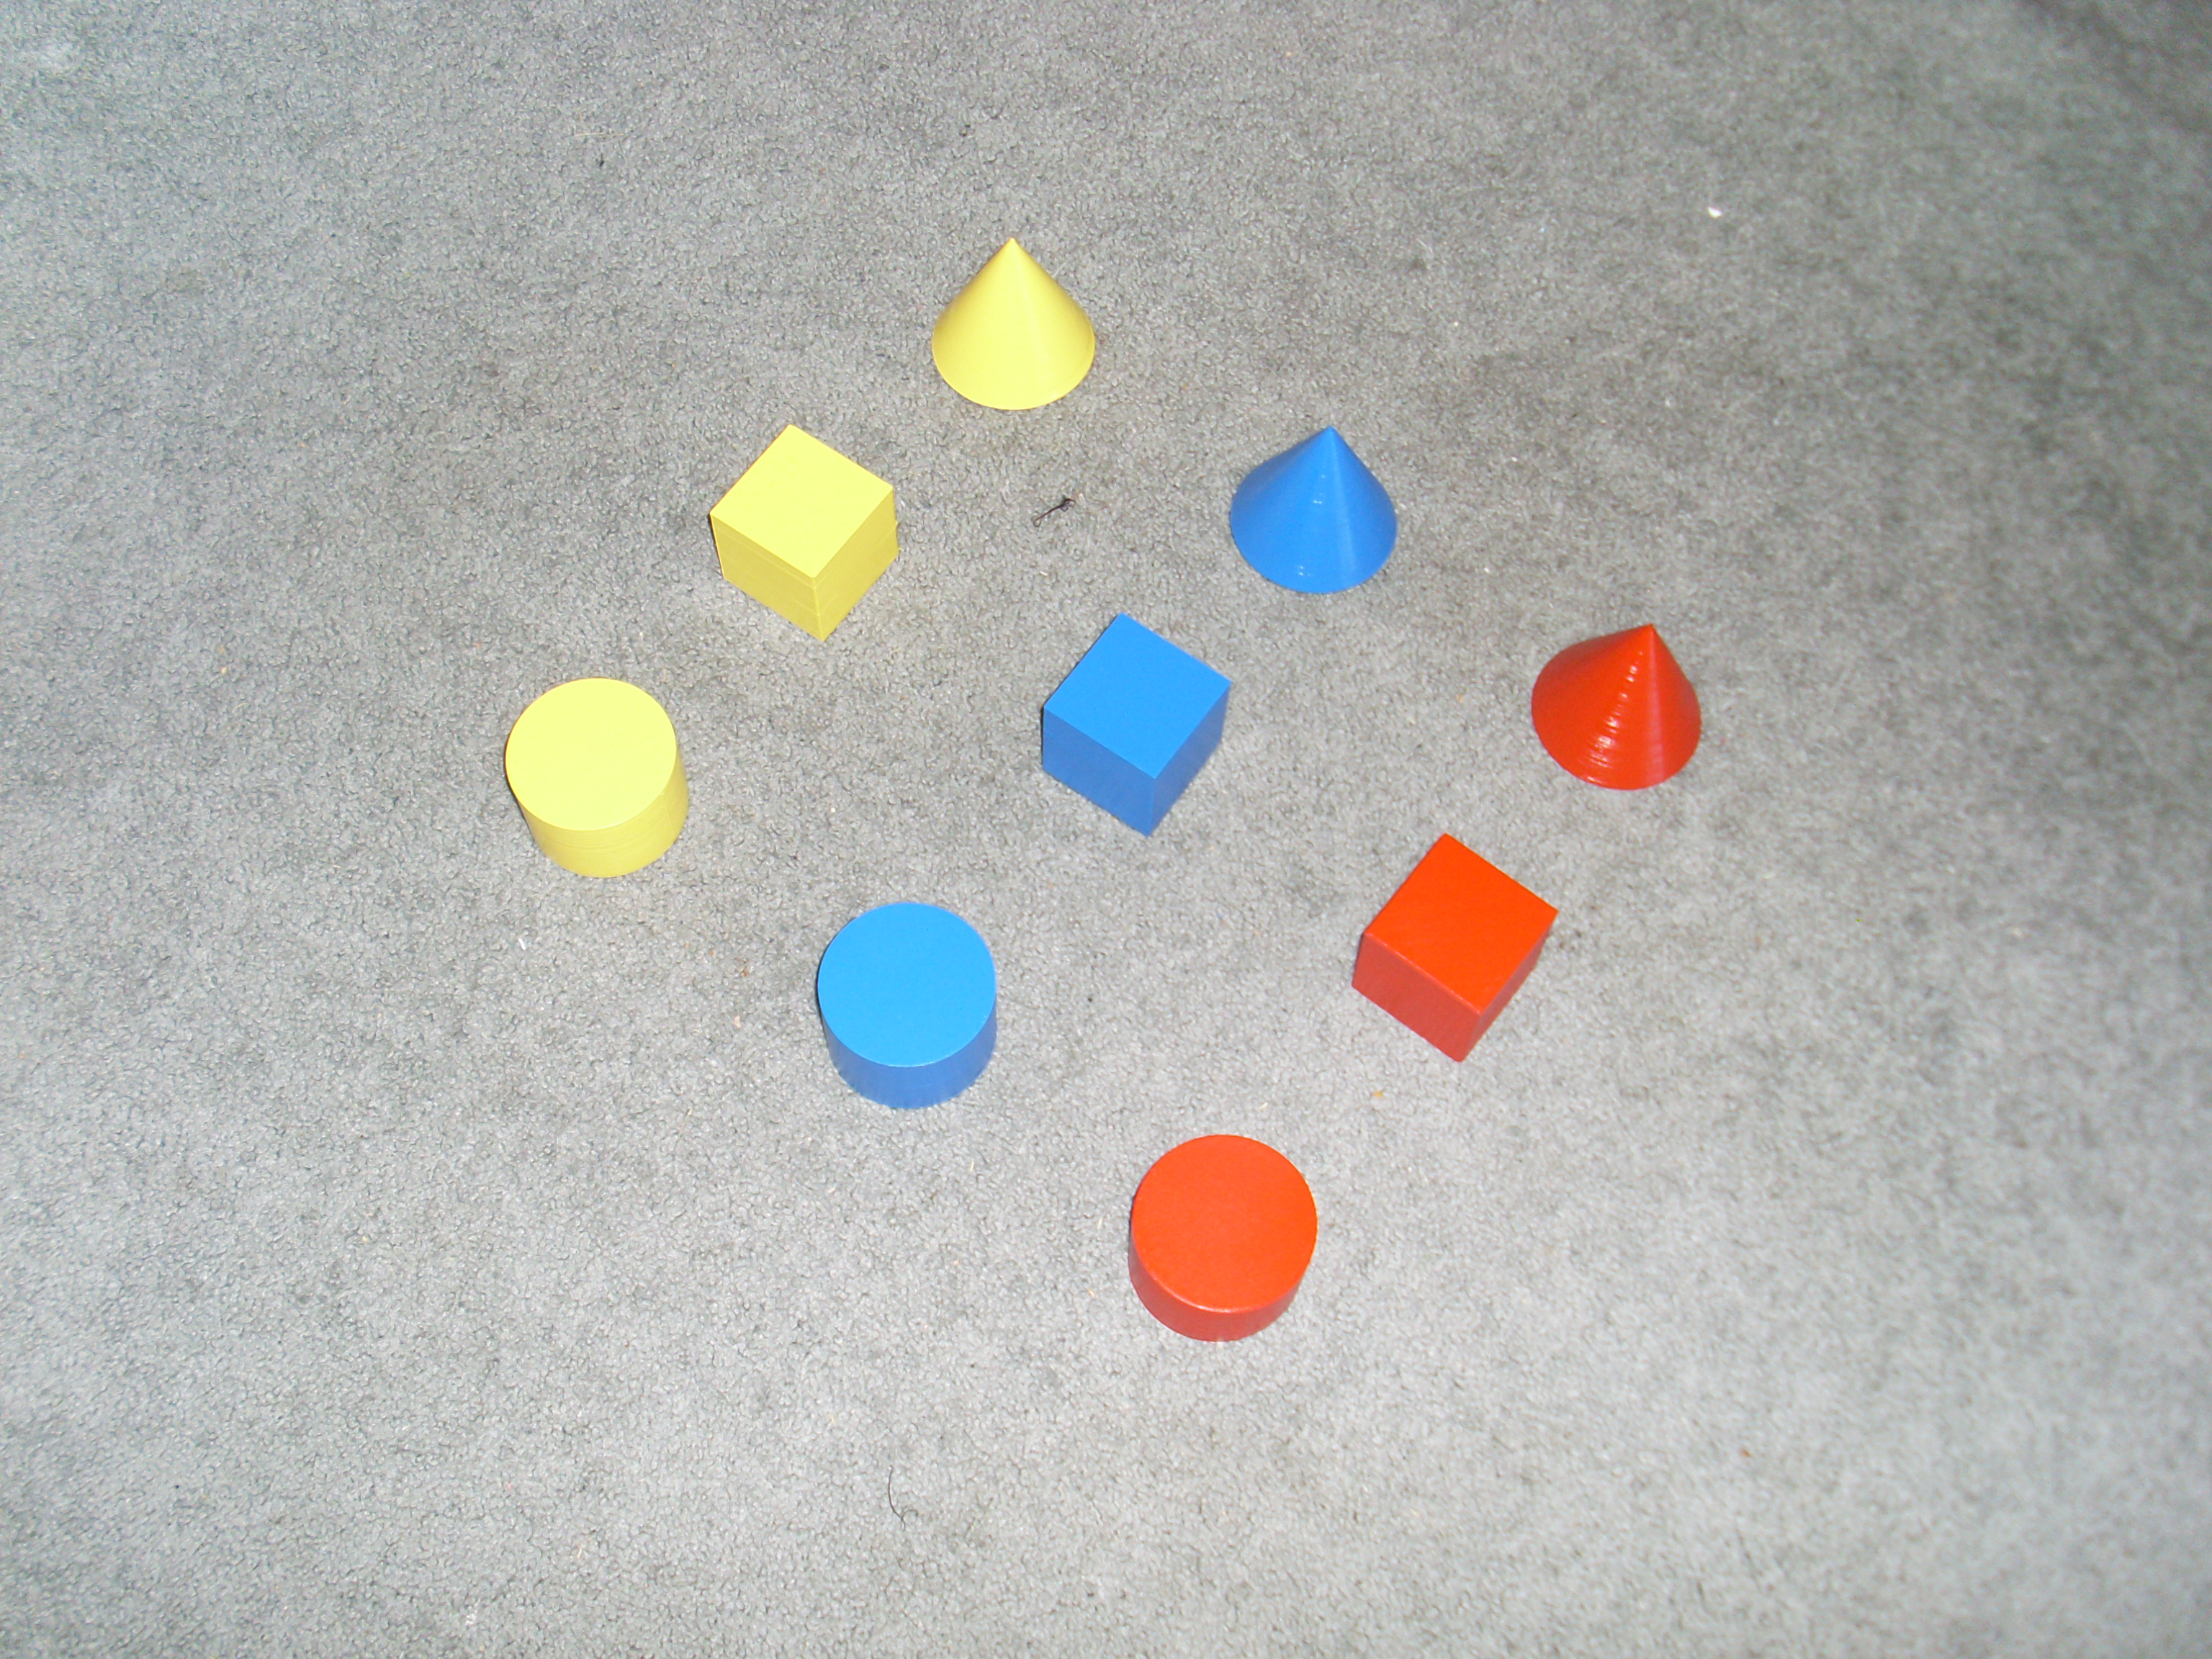
\includegraphics[width=100mm]{test_objects.JPG}
	\caption{Test Objects}
\end{figure}

We used the following angles/distances for capturing the objects:

\begin{tabular}{c c c c}
	Z Angle & Orthogonal Distance To Object & Height Offset \\
	\hline
	0 & ~18-32 in & 0 \\
	45 & ~18-32 in & 0 \\
	90 & ~18-32 in & 0 \\
	135 & ~18-32 in & 0 \\
	180 & ~18-32 in & 0 \\
	225 & ~18-32 in & 0 \\
	270 & ~18-32 in & 0 \\
	315 & ~18-32 in & 0 \\
	0 & ~18-32 in & 10 in \\
	45 & ~18-32 in & 10 in \\
	90 & ~18-32 in & 10 in \\
	135 & ~18-32 in & 10 in \\
	180 & ~18-32 in & 10 in \\
	225 & ~18-32 in & 10 in \\
	270 & ~18-32 in & 10 in \\
	315 & ~18-32 in & 10 in \\
	0 & 0 & ~36-48 in \\
\end{tabular}

The camera we used to capture the images was a Samsung L730. We used auto-focus and disabled flash.

We took pictures of the train objects in six diverse locations, four indoor locations with a variety of backgrounds (carpet, hardwood floor, vinyl, concrete) and two outdoor locations (concrete and grass). The outdoor pictures were taken in the early afternoon.

\subsection{Models}

Selecting models, as with most deep-learning tasks, involved some level of trial and error. Since we wanted to explore the efficacy of transfer learning for this task, we picked a variety of pre-existing image classification networks to see if any would perform better for the task:

\begin{enumerate}
	\item Xception \cite{chollet16}
	\item VGG16 \cite{simonyan14}
	\item VGG19 \cite{simonyan14}
	\item ResNet50 \cite{he15}
	\item InceptionV3 \cite{szegedy15}
	\item InceptionResNetV2 \cite{szegedy16}
	\item MobileNet \cite{howard}
	\item DenseNet \cite{huang16}
\end{enumerate}

We also decided to peel off several layers of the networks to gain access to higher-dimension feature spaces which might be necessary for such a complicated task. We tried to pick layers strategically, such as after a block of the model's calculations:

\begin{enumerate}
	\item Xception: \{0, 8\}
	\item VGG16: \{0, 3, 8\}
	\item VGG19: \{0, 3, 9\}
	\item ResNet50: \{0, 3, 13\}
	\item InceptionV3: \{0, 2, 19\}
	\item InceptionResNetV2: \{0, 5, 20\}
	\item MobileNet: \{0, 13, 20\}
	\item DenseNet: \{0, 3, 10\}
\end{enumerate}

Importantly, before inputting the data into our own model, we applied a standard scalar transformation (trained on the output of the training data from the transfer model), then a normalization operation. Our reasoning was that such operations seemed to reduce the chance that the model would learn the all 0's classifier.

For our own model, we opted for a densely-connected network. Our reasoning behind that decision was that, since the transfer models used convolutional layers, much of the image information will have already been processed at the point where our model is used. Thus, our model did not need convolutional layers.

We varied the number of dense layers between 1, 3 and 4 and the number of neurons per layer between 500, 1000, and 1500. Experimentally, this seemed like a good balance, as adding more layers and neurons tended to make our network learn the all 0's classifier.

To see if there was a point at which the test data reached a maximum accuracy, we trained each generated network for 10 epochs.

Additional Settings:

\begin{itemize}
	\item Optimization Algorithm: Adam. The reason for this decision is that Adam is an improvement over SGD for this type of application. From the literature, it sounds that Adam also has some automatic parameter estimation, as well.
	\item Loss Function: Binary Crossentropy. This is necessary for multi-label classification
	\item Inner Layer Activations: ReLU. ReLU performs better than other activation functions in most situations.
	\item Last Layer Activations: Sigmoid. This is necessary for multi-label classification
\end{itemize}

\section{Conclusion}

Our findings were that many model configurations descended to the all-0's output model. We observed that, as the number of neurons per layer and number of densely connected layers in our network increased, the probability of descending to the all-0's output model approached 1. However, some model configurations were able to improve accuracy on the training data, but no model was able to find any connection between the training data and testing data; as the training accuracy increased, test accuracy was inversely affected.

One possibility for this outcome is that we didn't collect enough data to allow the network to learn the abstractions of the various characteristics. Although the network was able to improve on the training set some, the network was unable to apply this learning to any of the test sets.

Another possibility is that such a complicated task requires a specially-built convolutional neural network. Whereas we used a transfer learning approach, image classification and object characteristic enumeration could be so different that we cannot transfer the knowledge of image classification networks to the task of object characteristic enumeration.

Unfortunately, as neural networks are a black-box model, it is difficult to know for certain the reason that our approach did not work, although the presentation of a working model may shed light onto the task (see below).

\subsection{Results}

Selected results are below. Note that none performed remarkably better than the all 0's classifier.

\begin{figure}[h!]
	\centering
	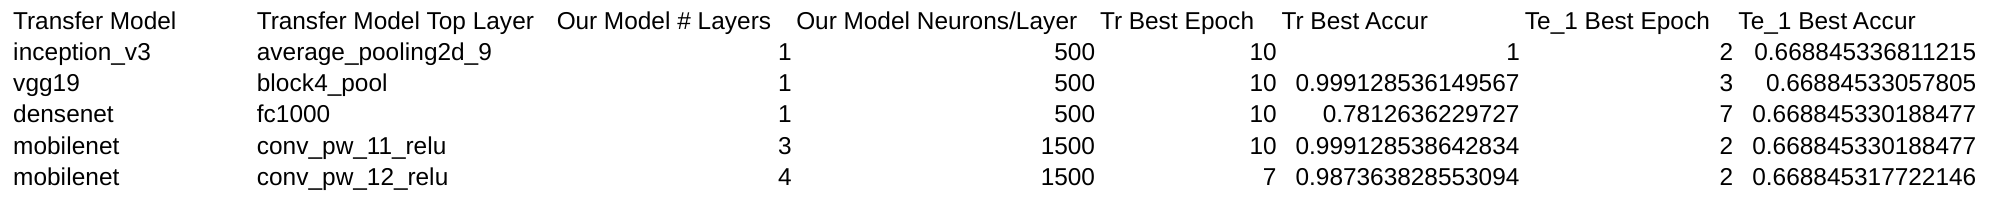
\includegraphics[width=160mm]{results_te_1.png}
	\caption{The model configurations with the best $ Te_1 $ accuracy}
\end{figure}

\begin{figure}[h!]
	\centering
	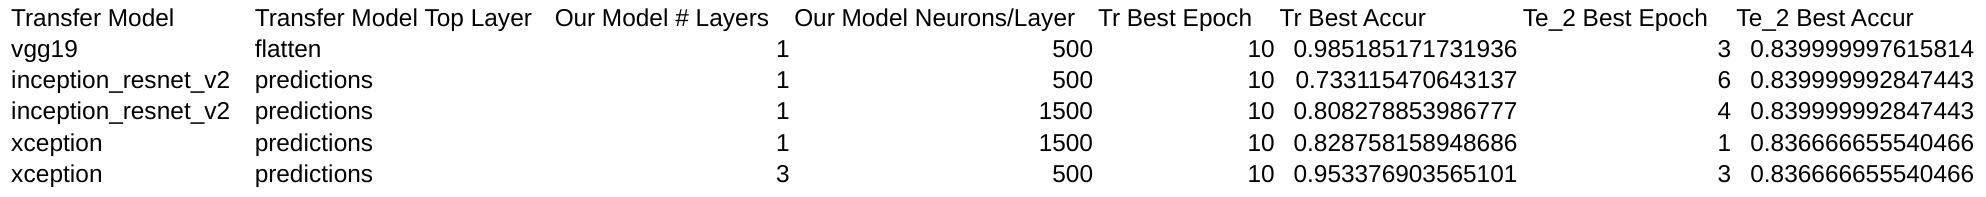
\includegraphics[width=160mm]{results_te_2.png}
	\caption{The model configurations with the best $ Te_2 $ accuracy}
\end{figure}

\begin{figure}[h!]
	\centering
	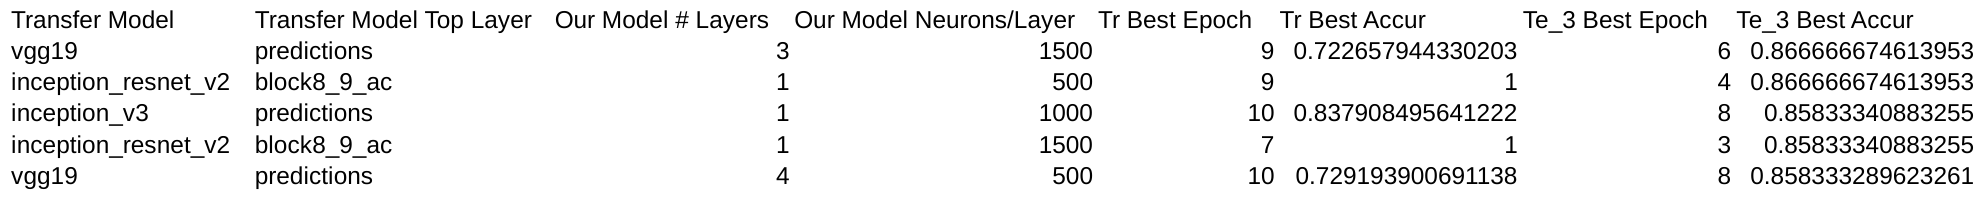
\includegraphics[width=160mm]{results_te_3.png}
	\caption{The model configurations with the best $ Te_3 $ accuracy}
\end{figure}

Figures 5 and 6 below illustrate the typical behavior of many of our generated models.

\begin{figure}[h!]
	\centering
	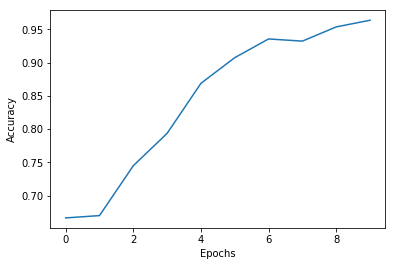
\includegraphics[width=100mm]{xception_0_4_2500_training_accur.png}
	\caption{$ Tr $ accuracy for the model using "Xception," 0 peeled layers, with our model having 4 dense layers and 2500 neurons per layer}
\end{figure}

\begin{figure}[h!]
	\centering
	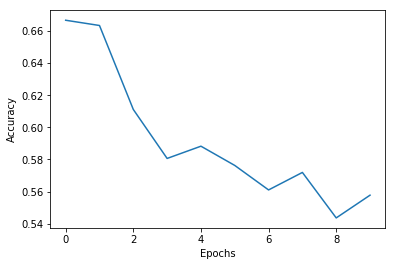
\includegraphics[width=100mm]{xception_0_4_2500_test_accur.png}
	\caption{$ Te_1 $ accuracy for the model using "Xception," 0 peeled layers, with our model having 4 dense layers and 2500 neurons per layer}
\end{figure}

\subsection{Recommended Further Work}

\subsubsection{Experimenting with More Training and Test Data}

Though nearly a thousand pictures were taken, the objects were only captured from several angles (17) and in several locations (6). This could have been detrimental to the model, as, without enough training examples, the model may not learn to abstract the characteristics of the objects. We recommend that further work augment the data more. One method would be to use a webcam and capture a video of each object from a full 360-degree arc. Another method would be to use more locations, or even capture an object as it is moving through locations, for example, being held in a hand as the person holding the object walks around.

\subsubsection{Create a CNN Specially Optimized for this Task}

Though we opted to make use of existing networks, this may have been a hindrance rather than a benefit. Such a complicated task may demand a network that is optimized for the task, rather than transfer learning from the output of an image classification network. An experiment with a carefully-constructed convolutional neural network may bring insight as to whether transfer learning is helpful or necessary for this task.

\subsubsection{Embodying the Model in a Robotic Agent}

The original motivation of this work was to, eventually, incorporate capturing an object from a variety of angles into a robotic agent to allow it to learn in an interactive learning session with a human. However, improvements to the model should be made before attempting this.

\begin{thebibliography}{99}

\bibitem{goodfellow16}
	Ian Goodfellow, Yoshua Bengio, Aaron Courville. 
	\textit{Deep Learning}, 
	The MIT Press, 
	Cambridge, MA, 
	1st Ed.,
	2016.
	
\bibitem{chollet16}
	François Chollet.
	"Xception: Deep Learning with Depthwise Separable Convolutions,"
	Cornell University Library,
	2016.
	https://arxiv.org/abs/1610.02357
	
\bibitem{simonyan14}
	Karen Simonyan, Andrew Zisserman.
	"Very Deep Convolutional Networks for Large-Scale Image Recognition,"
	Cornell University Library,
	2014.
	https://arxiv.org/abs/1409.1556
	
\bibitem{he15}
	Kaiming He, Xiangyu Zhang, Shaoqing Ren, Jian Sun.
	"Deep Residual Learning for Image Recognition,"
	Cornell University Library,
	2015.
	https://arxiv.org/abs/1512.03385
	
\bibitem{szegedy15}
	Christian Szegedy, Vincent Vanhoucke, Sergey Ioffe, Jonathon Shlens, Zbigniew Wojna.
	"Rethinking the Inception Architecture for Computer Vision,"
	Cornell University Library,
	2015.
	https://arxiv.org/abs/1512.00567
	
\bibitem{szegedy16}
	Christian Szegedy, Sergey Ioffe, Vincent Vanhoucke, Alex Alemi.
	"Inception-v4, Inception-ResNet and the Impact of Residual Connections on Learning,"
	Cornell University Library,
	2016.
	https://arxiv.org/abs/1602.07261
	
\bibitem{howard}
	Andrew G. Howard, Menglong Zhu, Bo Chen, Dmitry Kalenichenko, Weijun Wang, Tobias Weyand, Marco Andreetto, Hartwig Adam.
	"MobileNets: Efficient Convolutional Neural Networks for Mobile Vision Applications,"
	Google, Inc.
	https://arxiv.org/pdf/1704.04861.pdf
	
\bibitem{huang16}
	Gao Huang, Zhuang Liu, Laurens van der Maaten, Kilian Q. Weinberger.
	"Densely Connected Convolutional Networks,"
	Cornell University Library,
	2016.
	https://arxiv.org/abs/1608.06993

\end{thebibliography}

\end{document}
